\documentclass[journal]{IEEEtran}
\usepackage[utf8]{inputenc}
\usepackage{amsmath}
\usepackage{amsfonts}
\usepackage{amssymb}
\usepackage{fancyhdr}
\usepackage{float}
\usepackage{multirow}
\usepackage[pdfborder={0 0 0}]{hyperref}
\usepackage[ampersand]{easylist}
\usepackage{longtable}
\usepackage{tabularx}
\usepackage{booktabs}
\usepackage[activeacute,spanish]{babel}
\usepackage[pdftex]{graphicx}
\usepackage{amssymb}
\usepackage{color}
\usepackage{listings}
\hyphenation{op-tical net-works semi-conduc-tor}
\begin{document}
%
% paper title
\title{Instalación del firmware OpenWsn dentro de OpenMotes y configuración de OpenWrt para su uso}
\author{Tomás Lagos, Estudiante ingeniería civil en informática y telecomunicaciones}
        
\markboth{Intalación~del~firmware~OpenWsn~dentro~de~OpenMotes~y~configuración~de~OpenWrt~para~su~uso,~Vol.~1, No.~1,~02~Junio~2016}{Shell \MakeLowercase{\textit{et al.}}: Bare Demo of IEEEtran.cls for Journals}
\maketitle
\IEEEpeerreviewmaketitle
\section{Introducción}
Los OpenMotes son dispositivos, los cuales se componen de las siguientes piezas que se muestran a continuación:
\begin{itemize}
        \item OpenMote-CC2538: El openMote-CC2538 es el núcleo del hardware el cual contiene el firmware OpenWsn. Este posee un conector de antena y un chip de sistema CC2538 entre otros.
        \begin{figure}[!ht]
			\begin{center}
			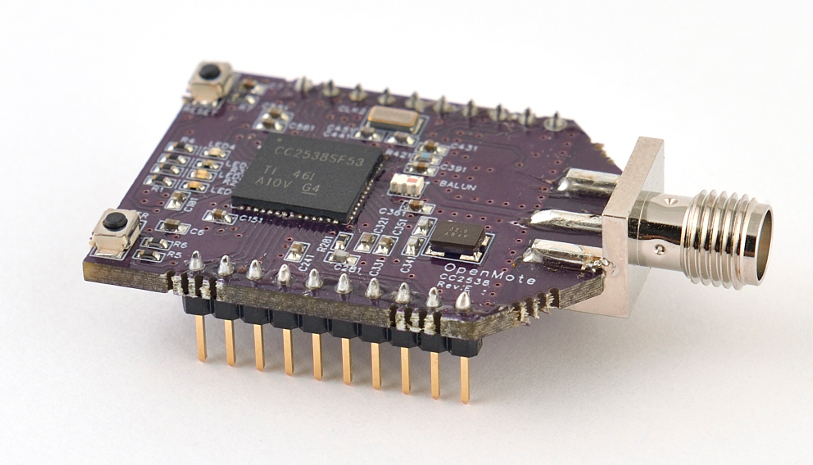
\includegraphics[scale=0.5]{motecc2538.jpg}
			\end{center}			            
			\caption{OpenMote-CC2538.}        
        \end{figure}
        
        \item OpenBattery: El OpenBattery es la plataforma que le entrega energía al OpenMote-CC2538. Este tiene dos entradas para pilas AAA. Además de tres sensores, los cuales son de humedad y temperatura, aceleración y de luz.
        \begin{figure}[!ht]
			\begin{center}
			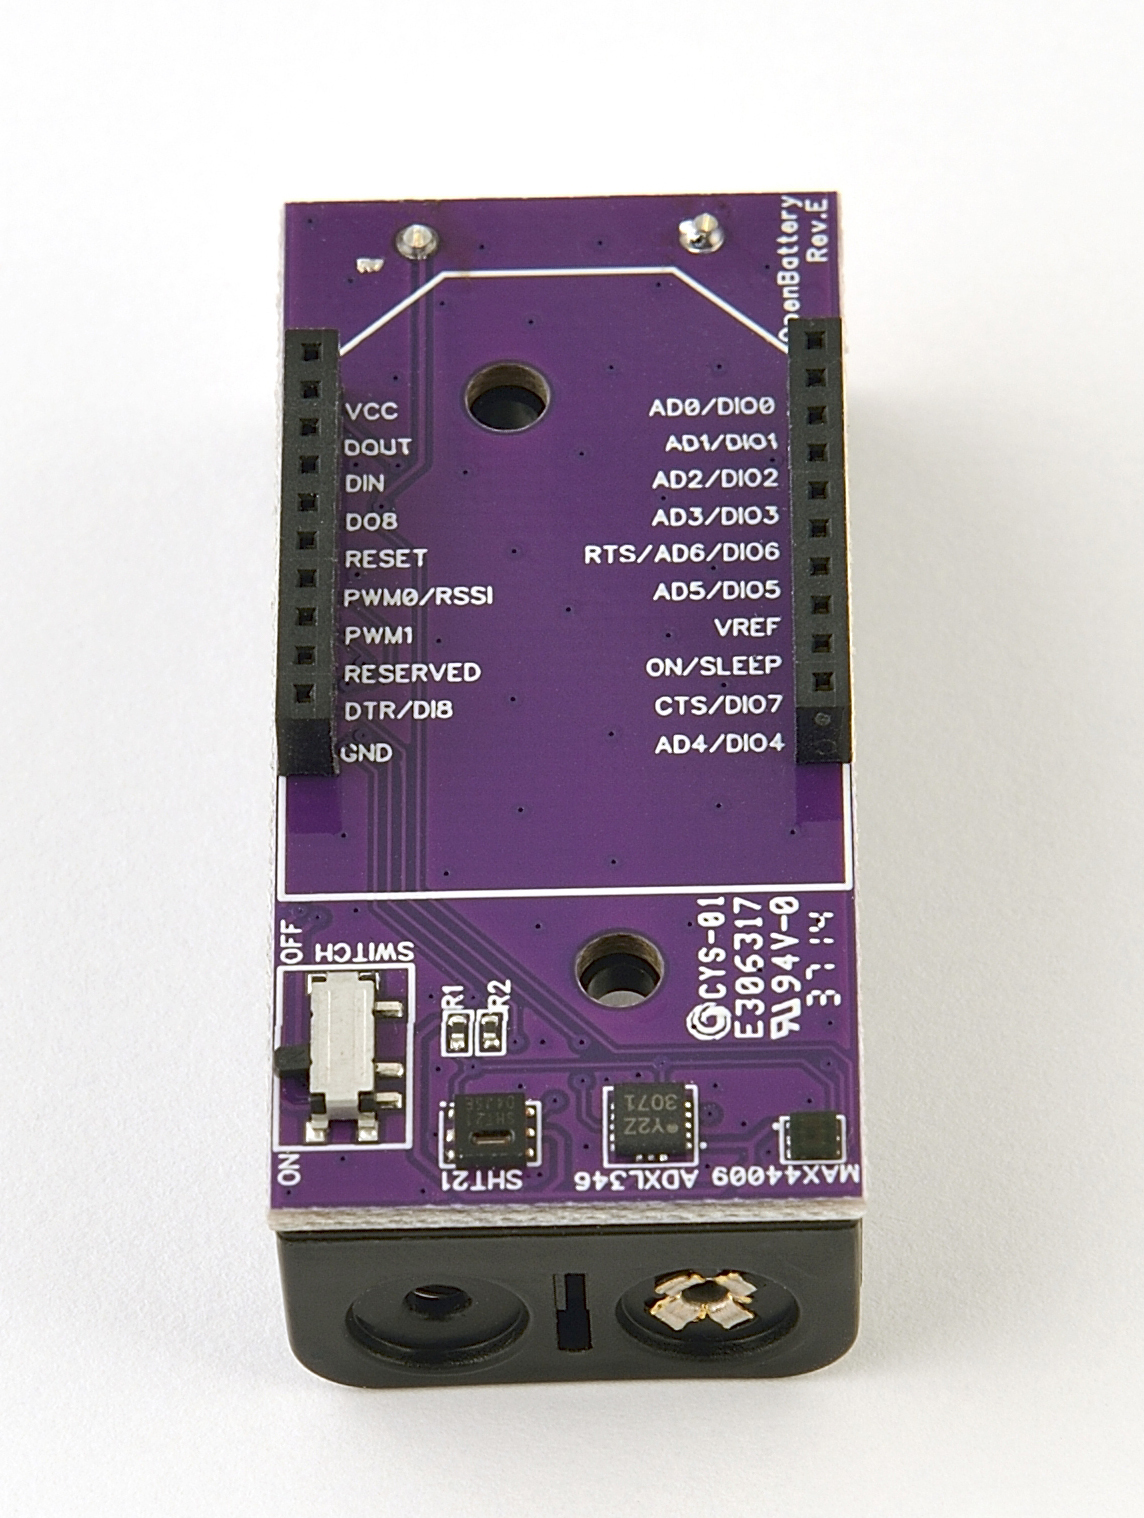
\includegraphics[scale=0.3]{openbattery.jpg}
			\end{center}			            
			\caption{OpenBattery.}        
        \end{figure}
        \item OpenBase: El OpenBase es la plataforma que permite la comunicación de los motes existentes con el equipo.
        \begin{figure}[!ht]
			\begin{center}
			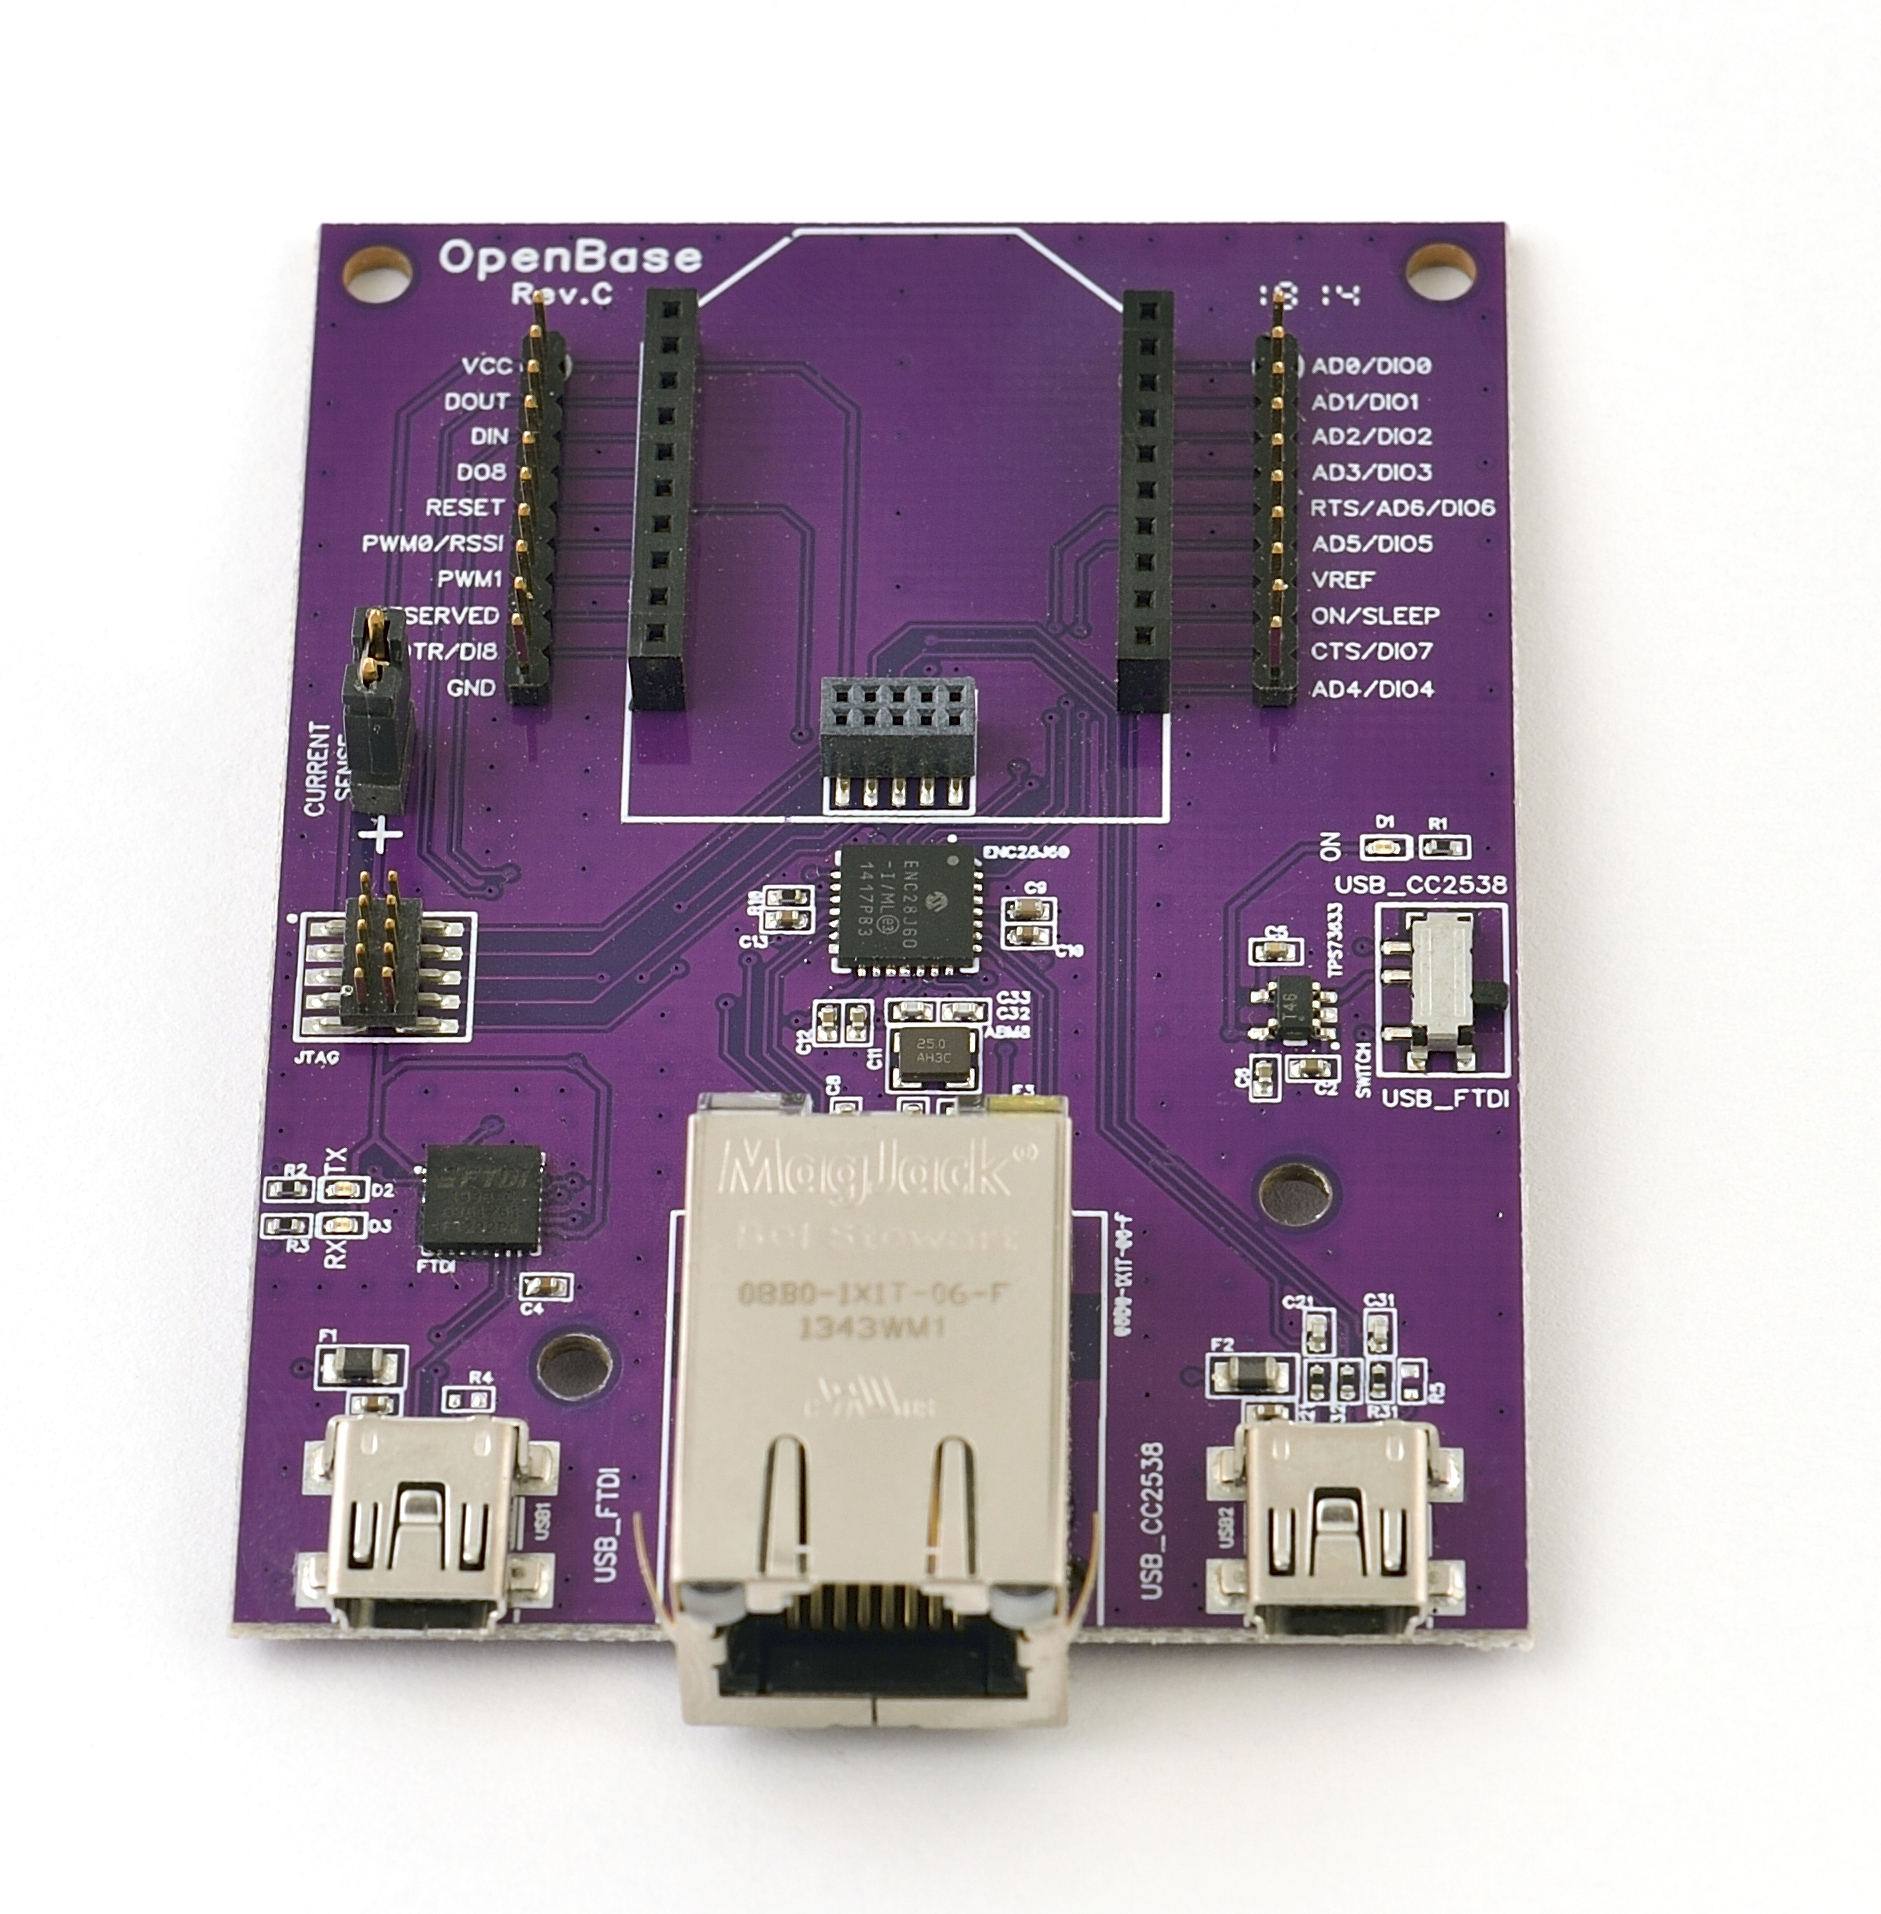
\includegraphics[scale=0.23]{openbase.jpg}
			\end{center}			            
			\caption{OpenBase.}        
        \end{figure}   
\end{itemize}
Los dispositivos OpenMote-CC2538 tendrán instalados el firmware OpenWsn, el cual está elaborado para fines experimentales.
\\
En este informe se explica, cómo se realiza la instalación del OpeWsn dentro de un OpenMode, como lograr su funcionamiento dentro de un equipo con OpenWrt incorporado y realizar una comunicación ICMP entre los Motes existentes hacia el OpenWrt y de este hacia un equipo.
\section{Instalación del OpenWsn dentro del OpenMote}
Para la instalación del OpenWsn se utilizará la guía https://openwsn.atlassian.net/wiki/display/OW/Kickstart+Linux.
\\
El primer paso para la instalación del OpenWsn, es la descarga de los proyectos
\begin{itemize}
        \item OpenWsn-Sw: Se encuentran todos los softwares para iniciar OpenWsn.
        \item OpenWsn-fw: Se encuentran los firmwares compilados de OpenWsn.
\end{itemize}
Con los siguientes comandos:
\begin{lstlisting}[frame=single]
~$ cd Desktop/
~/Desktop$ mkdir openwsn
~/Desktop$ cd openwsn/
~/Desktop/openwsn$ git clone https://githu
b.com/openwsn-berkeley/openwsn-fw.git
~/Desktop/openwsn$ git clone https://githu
b.com/openwsn-berkeley/openwsn-sw.git   
\end{lstlisting}
Ademas de los paquetes adicionales que se muestran a continuación:
\begin{lstlisting}[frame=single]
~$ sudo apt-get install python-dev      
~$ sudo apt-get install python-pip
~$ sudo pip install bottle
~$ sudo pip install PyDispatcher
~$ sudo apt-get install scons
\end{lstlisting}
\newpage
Ya teniendo los pre-requisitos instalados, se emplea a la compilación del firmware. Para lograr esto, se debe dejar el OpenMote en estado BootLoader y para luego compilar el firmware. Para entrar al estado Bootloader se debe conectar el OpenMote-CC2538 al OpenBase y luego conectar el pin On/Sleep con el pin GND. 
\begin{figure}[!h]
	\begin{center}
		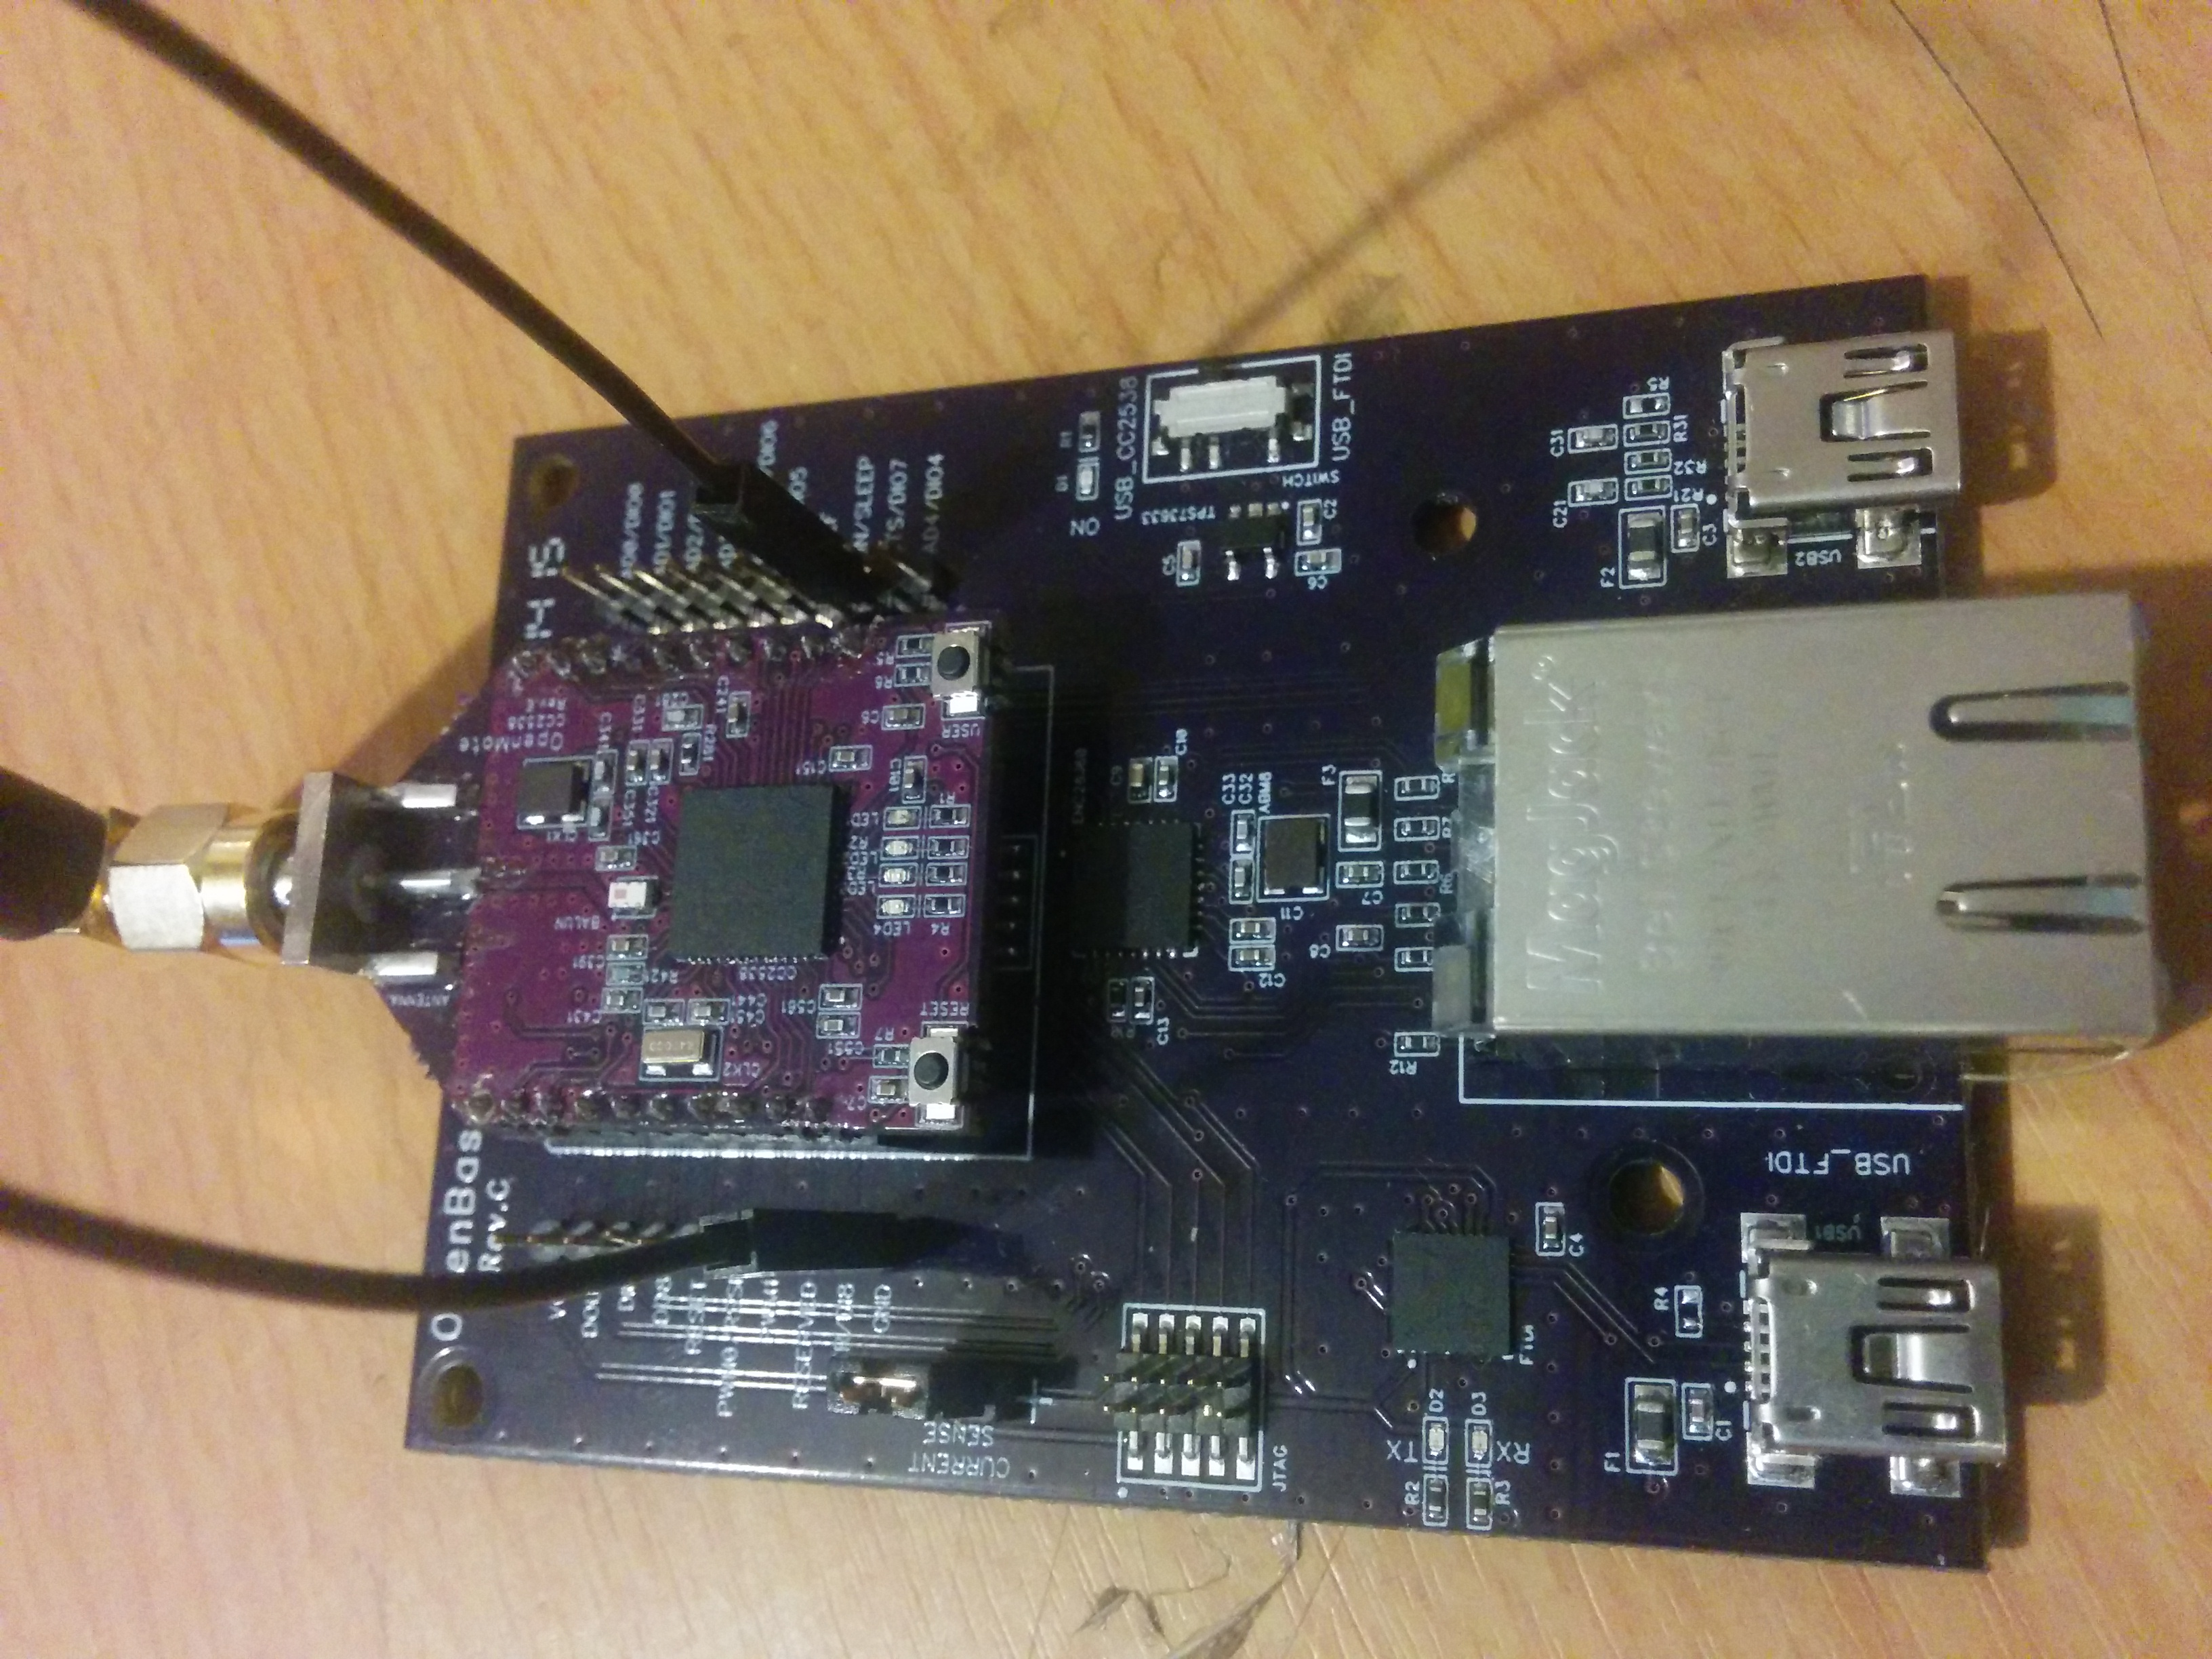
\includegraphics[scale=0.05]{bootloader.jpg}
	\end{center}			            
	\caption{OpenBase.}        
\end{figure}

De esta manera solo queda insertar los siguientes códigos:
\begin{lstlisting}[frame=single]
~$ cd openwsn-fw        
~$ sudo scons board=OpenMote-CC2538
toolchain=armgcc goldenImage=root
bootload=/dev/ttyUSB0 oos_openwsn
\end{lstlisting}
Cabe mencionar que el parámetro bootload debe referirse a la dirección del puerto serial. En este caso ttyUSB0.
Esto debe repetirse con todos los motes con los que se quiere trabajarán.
\ \\
El siguiente paso, es correr el OpenWsn bajo el software openVisualizerWeb. Para efectuarlo se requiere utilizar los siguiente Comandos:
\begin{lstlisting}[frame=single]
~$ cd openwsn-sw/software/openvisualizer/
~$ cd bin/openVisualizerApp/
~$ sudo python openVisualizerWeb.py
\end{lstlisting}
Luego se accede a la url http://localhost:8080 donde se visualizará la siguiente página.
\\
\begin{figure}[!ht]
	\begin{center}
		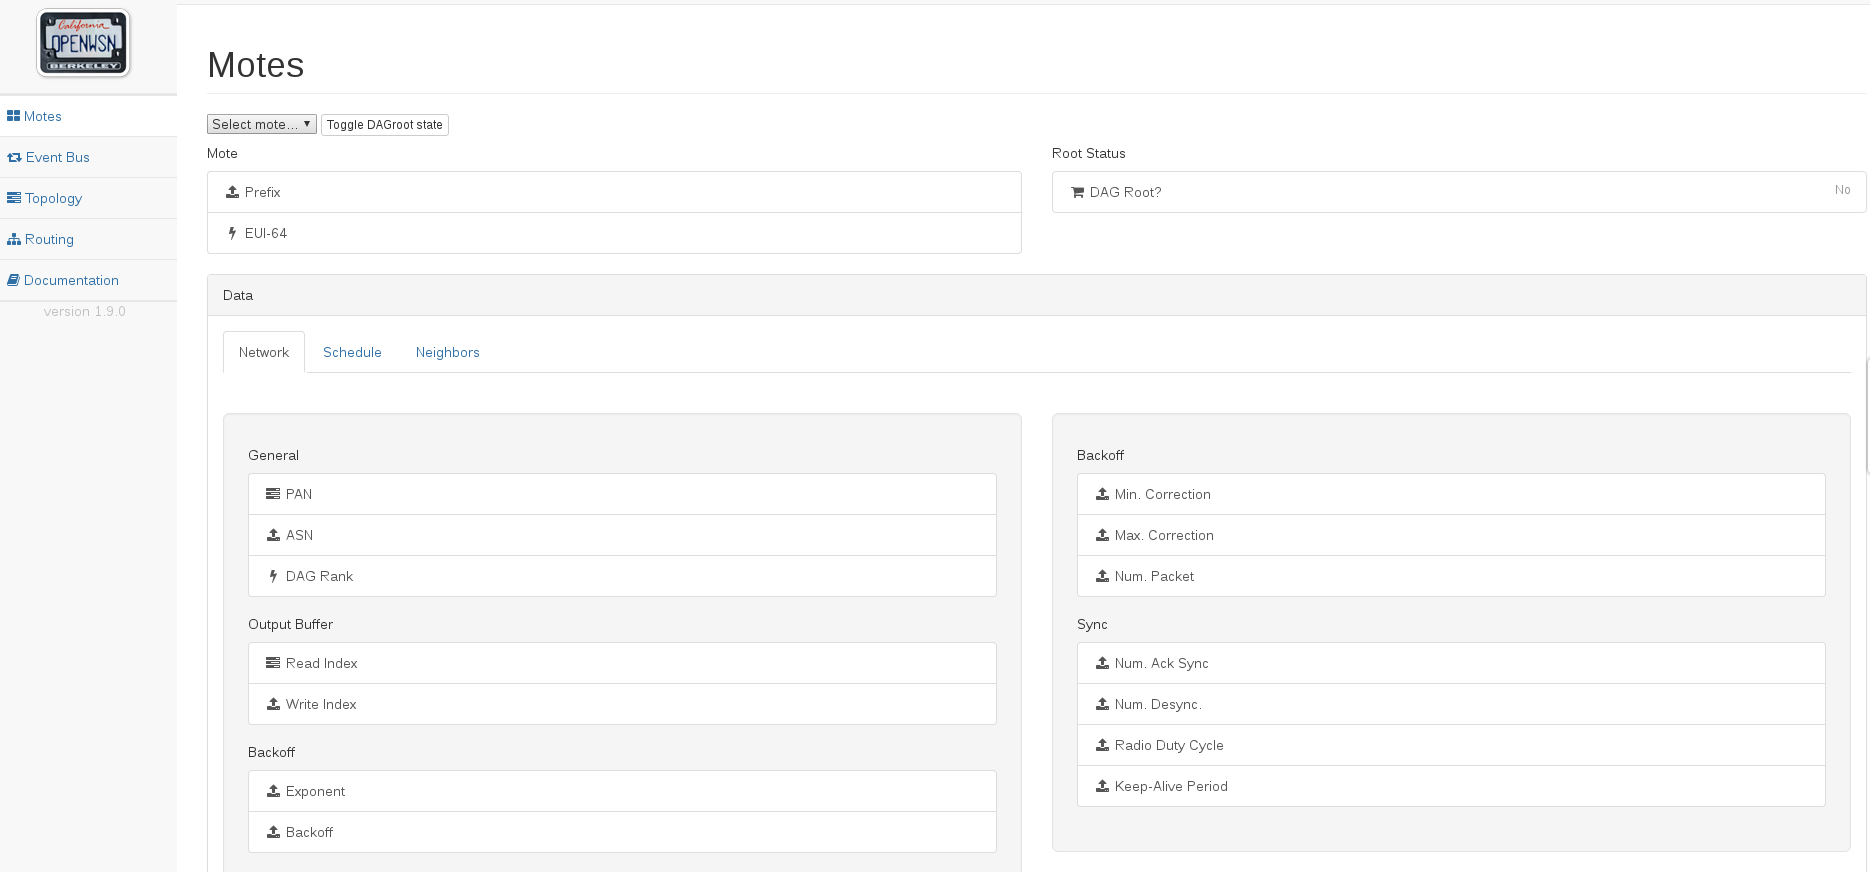
\includegraphics[scale=0.13]{openweb.png}
	\end{center}			            
	\caption{OpenVisualizerWeb}        
\end{figure}
\newpage
Se selecciona el mote y se incorpora como DAG Root
\\
\begin{figure}[!ht]
	\begin{center}
		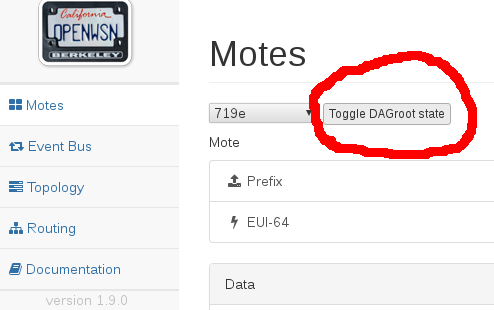
\includegraphics[scale=0.45]{dagroot.png}
	\end{center}			            
	\caption{DAGroot}        
\end{figure}
\\
\section{Configuración de OpenWrt para la comunicación de OpenWsn}  
 Esta configuración se realizó con el firmware de Openwrt Chaos Calmer 15.05.1
 \\
  
 El primer paso es la instalación de las siguientes paquetes y dependencias de python.
 \begin{lstlisting}[frame=single]
~$ opkg update
~$ opkg install python-light
~$ opkg install python-pip
~$ pip install bottle
~$ pip install PyDispatcher
~$ pip install PySerial
\end{lstlisting}
\ \\
Y la instalación de las dependencias serial usb y tun con los siguientes comandos
 \begin{lstlisting}[frame=single]
~$ opkg install python-light
~$ opkg install python-pip
~$ opkg install kmod-usb-serial
~$ opkg install kmod-usb-serial-ftdi
~$ opkg install kmod-usb-serial-option
~$ opkg install kmod-usb-serial-pl2303
~$ opkg install kmod-usb-serial-wwan
~$ opkg install kmod-usb2
~$ opkg install kmod-tun
\end{lstlisting}
\
Ya teniendo los driver y softwares necesarios se emplea la configuración Network de openwrt, el cual se encuentra ubicado en /etc/config/network. 
\newpage 
El archivo debe considerar los siguientes parámetros:
 \begin{lstlisting}[frame=single]
config interface 'lan'
        option ifname 'eth0'
        option proto 'static'
        option ipaddr   '192.168.0.1'   
        option netmask  '255.255.255.0'
        option ip6assign '64'
        option ip6addr 'aaaa::2/64'
        option ip6gw    'aaaa::1'
        
config interface 'openwsn'
        option ifname 'tun0'
        option _orig_ifname 'tun0'
        option _orig_bridge 'false'
        option proto 'static'
        option ip6assign '64'
        option ip6addr  'bbbb::1/64'
\end{lstlisting}
\
Donde la interfaz Lan se le asignará la IPv6 aaaa::1. Ademas se genera la creación de la interfaz Openwn, que poseerá la entrada tun0 del puerto serial y las IPv6 bbbb::1, dado que OpenWsn trabaja con ellas.
\ \\
El siguiente paso, es la configuración del archivo firewall, el cual se encuentra ubicado en la dirección /etc/config/firewall. Se considerarán los siguientes parámetros para su configuración:
\begin{lstlisting}[frame=single]
config rule
        option name 'Allow-ICMPv6-Input'
        option proto 'icmp'
        list icmp_type 'echo-request'
        list icmp_type 'echo-reply'
        list icmp_type 'destination-
                        unreachable'
        list icmp_type 'packet-too-big'
        list icmp_type 'time-exceeded'
        list icmp_type 'bad-header'
        list icmp_type 'unknown-header-
                        type'
        list icmp_type 'router-
                        solicitation'
        list icmp_type 'neighbour-
                        solicitation'
        list icmp_type 'router-
                        advertisement'
        list icmp_type 'neighbour-
                        advertisement'
        option limit '1000/sec'
        option family 'ipv6'
        option target 'ACCEPT'
        option src '*'
        option dest '*'
\end{lstlisting}
\newpage
\begin{lstlisting}[frame=single]        
config zone
        option name 'openwsn'
        option input 'ACCEPT'
        option output 'ACCEPT'
        option forward 'ACCEPT'
        option masq '1'
        option mtu_fix '1'
config forwarding
        option dest 'openwsn'
        option src 'lan'
config forwarding
        option dest 'lan'
        option src 'openwsn'
\end{lstlisting}
Se observa la creación de los cofig zone, y de los config forwarding además de la modificación del ``rule'' con los ``option src '*' '' y ``dest '*' ''
\ \\
Cabe señalar que para la utilización del OpenWsn se debe incorporar la carpeta openwsn-sw dentro de la carpeta /root/
\section{Instalación de OpenWrt dentro de una Raspberry Pi 2 y la configuración del firmware OpenWsn para su funcionamiento}
El firmware disponible para la raspberry pi para OpenWrt se encuentra en el siguiente link:
http://downloads.openwrt.org/chaos\_calmer/15.05.1/brcm2708/bcm2709/
\\
Para poder instalar el firmware a la Paspberry Pi 2, se debe ingresar la tarjeta SD dentro del equipo. Luego se utiliza el siguiente comando:
\begin{lstlisting}[frame=single]
dd if=/home/username/Downloads/openwrt-
brcm2708-bcm2709-sdcard-vfat-ext4.img
 of=/dev/sdX bs=2M conv=fsync
\end{lstlisting}
Donde el Sdx es la ubicación donde se encuentra montado la tarjeta SD
\ \\
Se debe utilizar todas las configuraciones del capítulo III
\ \\
Dado que la Raspberry cuenta con recursos limitados, se debe modificar el parámetro RX del Schedule dentro del Firmware de OpenWsn ubicado en openwsn-fw/openstack/schedule.h y modificar NUMSERIALRX 3,  por NUMSERIALRX 5. Se debe recompilar el nuevo firmware a todos los motes que se utilizarán para trabajar.
\section{Comunicación entre un equipo a un mote entremedio de OpenWrt}
Para generar la comnicación entre un equipo a un mote, la raspberry debera estar conectada mediante el cable serial USB hacia el Openbase y el puerto ethernet a el puerto ethernet del equipo. De esta manera la Raspberry funcionara como router entre los dos equipos.
\\

Para ver la interacción entre los equipos, se genera un ping con un header de 10 bits hacia cualquera de los distintos motes que existen, exceptuando el Mote conectado al Openbase.   
\end{document}
